%   Il progetto nasce dal template per il frontespizio realizzato da Marco Antonio Corallo, che ringrazio. Seguono alcuni commenti per evidenziare la presenza di alcuni pacchetti che mi sono stati utili per la stesura della tesi. Chiaramente, dipende tutto dal tipo di lavoro che uno vuole eseguire, che determina anche le diverse esigenze. Durante la stesura ho passato molto tempo su siti e forum a cercare di risolvere alcuni probelmi di formattazione, ma in generale Latex è stato piuttosto versatile. 

% Tipo di documento. L'uso di twoside implica che i capitoli inizino sempre con la prima pagina a sinistra, eventualmente lasciando una pagina vuota nel capitolo precedente. Se questa cosa è fastidiosa, è possibile rimuoverlo. 
\documentclass[a4paper, twoside,openright]{report}
\usepackage{siunitx}

\DeclareMathSizes{10}{10}{7}{4}

% Dimensione dei margini
\usepackage[a4paper,top=3cm,bottom=3cm,left=3cm,right=3cm]{geometry} 
% Dimensione del font
\usepackage[fontsize=13pt]{scrextend}
% Lingua del testo
\usepackage[english,italian]{babel}

\usepackage{natbib}
% \bibpunct{(}{)}{;}{a}{}{,} % to follow the A&A style

% Lingua per la bibliografia
\usepackage[fixlanguage]{babelbib}
% Codifica del testo
\usepackage[utf8]{inputenc} 
% Encoding del testo
\usepackage[T1]{fontenc}


% Permette di generare testo fittizio. Mi è stato utile 
% per capire quale sarebbe stata l'impostazione del 
% testo nella pagina prima che scrivessi un determinato paragrafo
\usepackage{lipsum}
% Per ruotare le immagini
\usepackage{rotating}
% Per modificare l'header delle pagine 
\usepackage{fancyhdr}    
\usepackage{booktabs}
\usepackage{float}

% Librerie matematiche
\usepackage{amssymb}
\usepackage{amsmath}
\usepackage{amsthm} 
\usepackage{accents}
\usepackage{aas_macros}
\usepackage{garamondlibre}
\usepackage{newtxmath}  % matematica

% Uso delle immagini
\usepackage{graphicx}
% Uso dei colori
\usepackage[dvipsnames]{xcolor}         
% Uso dei listing per il codice
\usepackage{listings}          
% Per inserire gli hyperlinks tra i vari elementi del testo 
\usepackage{hyperref}     
% Diversi tipi di sottolineature
\usepackage[normalem]{ulem}

\usepackage{xspace}
% -----------------------------------------------------------------

% Modifica lo stile dell'header
\pagestyle{fancy}
\fancyhf{}
\lhead{\rightmark}
\rhead{\textbf{\thepage}}
\fancyfoot{}
\setlength{\headheight}{12.5pt}

% Rimuove il numero di pagina all'inizio dei capitoli
\fancypagestyle{plain}{
  \fancyfoot{}
  \fancyhead{}
  \renewcommand{\headrulewidth}{0pt}
}

% Stile del codice
\lstdefinestyle{codeStyle}{
    % Colore dei commenti
    commentstyle=\color{black},
    % Colore delle keyword
    keywordstyle=\color{black},
    % Stile dei numeri di riga
    numberstyle=\tiny\color{black},
    % Colore delle stringhe
    stringstyle=\color{black},
    % Dimensione e stile del testo
    basicstyle=\ttfamily\footnotesize,
    % newline solo ai whitespaces
    breakatwhitespace=false,     
    % newline si/no
    breaklines=true,                 
    % Posizione della caption, top/bottom 
    captionpos=b,                    
    % Mantiene gli spazi nel codice, utile per l'indentazione
    keepspaces=true,                 
    % Dove visualizzare i numeri di linea
    numbers=left,                    
    % Distanza tra i numeri di linea
    numbersep=5pt,                  
    % Mostra gli spazi bianchi o meno
    showspaces=false,                
    % Mostra gli spazi bianchi nelle stringhe
    showstringspaces=false,
    % Mostra i tab
    showtabs=false,
    % Dimensione dei tab
    tabsize=2
} \lstset{style=codeStyle}

% Stile di codice per dimensioni maggiori, in cui ho avuto bisogno di un testo più picolo (ad esempio se si vuole inserire del codice che ha linee molto lunghe). Per usare questo stile piuttosto che il precedente, usare 

% \lstset{style=longBlock}
%  % inserire il codice...
% \lstset{style=codeStyle}

% Il secondo comando consente di tornare allo stile precedente 
\lstdefinestyle{longBlock}{
    commentstyle=\color{black},
    keywordstyle=\color{black},
    numberstyle=\tiny\color{black},
    stringstyle=\color{black},
    basicstyle=\ttfamily\scriptsize,
    breakatwhitespace=false,         
    breaklines=true,                 
    captionpos=b,                    
    keepspaces=true,                 
    numbers=left,                    
    numbersep=5pt,                  
    showspaces=false,                
    showstringspaces=false,
    showtabs=false,                  
    tabsize=2
} \lstset{style=codeStyle}

% Togliendo il commento al comando che segue, si inseriscono nella bibliografia anche le fonti presenti in Bibliography.bib ma non citati direttamente con il comando \cite
% \nocite{*}

% Margini prima e dopo blocchi di codice, per avere più distanza
\lstset{aboveskip=20pt,belowskip=20pt}

% Modifica dello stile dei riferimenti, con il testo in cyano
%\hypersetup{
%    colorlinks,
%    linkcolor=CornflowerBlue,
%    citecolor=CornflowerBlue
%}

% Aggiunti definizioni, teoremi, linea e listing
\newtheorem{definition}{Definizione}[section]
\newtheorem{theorem}{Teorema}[section]
\providecommand*\definitionautorefname{Definizione}
\providecommand*\theoremautorefname{Teorema}
\providecommand*{\listingautorefname}{Listing}
\providecommand*\lstnumberautorefname{Linea}

\raggedbottom

%\newcommand{\cgs}[1]{{\textcolor{brown}[\textcolor{red}{\bf{GS: }}{ \textcolor{brown}{#1]}}}}             
%\newcommand{\cmc}[1]{{\textcolor{blue}[\textcolor{magenta}{\bf{MC: }}{ \textcolor{blue}{#1]}}}}


% User defined commands
\newcommand{\src}{MAXI J1816--195\xspace}

% -----------------------------------------------------------------
\begin{document}

\begin{titlepage}
\begin{figure}[!htb]
    \centering
    
\includegraphics[keepaspectratio=true,scale=0.5]{images/Frontespizio/download.png}
\end{figure}

\begin{center}
    \LARGE{Università degli Studi di Cagliari}
    \vspace{5mm}
    \\ \large{Facoltà di Scienze Matematiche, Fisiche e Naturali}
    \vspace{5mm}
    \\ \LARGE{Laurea Magistrale in Fisica}
\end{center}

\vspace{15mm}
\begin{center}
    {\LARGE{\bf Thesis Title}}
    
    % Se il titolo è abbastanza corto da stare su una riga, si può usare
    
    % {\LARGE{\bf Un fantastico titolo per la mia tesi!}}
\end{center}
\vspace{30mm}

\begin{minipage}[t]{0.47\textwidth}
	{\large{Relatore:}{\normalsize\vspace{3mm}
	\\ 
        \large{\textbf{Prof. Riccardo Murgia}}\vspace{3mm} \\
        {\large{Co-relatori:}{\normalsize\vspace{3mm}
 	\bf\\ 
        \large{Prof. Thomas Kupfer\vspace{1mm}\\
                     Weitian Yu}
    \normalsize\vspace{3mm}\bf}}}}\\ 
\end{minipage}
\hfill
\begin{minipage}[t]{0.47\textwidth}\raggedleft
	{\large{Candidato:}{\normalsize\vspace{3mm} \bf\\ \large{Gabriele Todde}}}
\end{minipage}

\vspace{30mm}
\hrulefill
\\\centering{\large{ANNO ACCADEMICO 2024/2025}}

\end{titlepage}

\begin{abstract}
\addcontentsline{toc}{chapter}{Abstract}
In recent years ground-based interferometers such as LIGO and Virgo opened the high-frequency window of the rapidly evolving gravitational wave astronomy.
Future space-based detectors, in particular the \textit{Laser Interferometer Space Antenna} (LISA), will extend gravitational wave detection into the low-frequency band, where Galactic compact binaries such as double white dwarfs (DWDs) are expected to shape LISA's sensitivity curve significantly;
the aim of this work is to investigate the expected gravitational wave background produced by \textit{extragalactic} DWDs in the local Universe, employing the \textit{Compact Object Synthesis and Monte Carlo Investigation Code} (\textbf{COSMIC}) to generate synthetic populations representing the galaxies included in the observational survey \textbf{Gravitational Wave Galaxy Catalog} (GWGC).
Each simulated binary contributes to the total gravitational wave strain, which is then combined across frequency bins and compared against the LISA sensitivity curve.
The results show that the total simulated extragalactic signal lies approximately one order of magnitude below LISA’s detection threshold, indicating that the noise from the unresolved sources will not produce a measurable imprint on the sensitivity curve.
Future developments could include the use of more advanced population synthesis codes and different prescriptions for binary evolution, or the extension of the analysis to larger observational galaxy catalogs and cosmological volumes.
\end{abstract}


\tableofcontents

% Rimuovere se non si vuole la tabella delle figure
% \listoffigures

%\chapter*{Introduction}
\addcontentsline{toc}{chapter}{Introduction}
In the context of the gravitational waves study, there are mainly two possible paths: the first is the \textbf{analysis of existing data} from experiments like Ligo, Virgo and Kagra, with the goal of detecting and characterizing the observable sources within their relative frequency bands;
the second is the \textbf{forecasting approach}, which aims to characterize future experiments in order to better understand what types of sources they could be able to detect and how well.
\vspace{2mm}\\
One of the most important future detectors is the European \textit{Laser Interferometer Space Antenna} (LISA), the first space-based gravitational wave detector. 
LISA will be arranged as an equilateral triangle with 2.5 million kilometers long arms, placed in a heliocentric orbit, and will operate within the frequency range from approximately $0.1\mathrm{mHz}$ to $1\mathrm{Hz}$. 
Among the typical sources that emit gravitational wave signal in this range are the \textbf{compact binaries}, and in our particular case we are interested in \textbf{double white dwarfs} (\textbf{DWDs}).
\vspace{2mm}\\
Many studies have been made to explore the effects of different type of sources on the LISA's sensitivity curve.
For example, we know that the unresolved binary Galactic systems produce a confusion gravitational wave foreground that shapes noticeably the curve close to its lowest threshold.
While the Galactic contribution has been extensively investigated, less attention has been devoted to the possible extragalactic binaries backgrounds.
Therefore, as a natural prosecution, the goal of this work is to estimate the gravitational wave background produced by the \textit{extragalactic} DWDs in the local universe, using the \textbf{COSMIC} code to generate synthetic astrophysical populations with the aid of the galaxies listed in the \textbf{Gravitational Wave Galaxy Catalog} (\textbf{GWGC}), an observational survey, as a reference.
The potential impact of these sources in the tentative to characterize the expected LISA sensitivity and to avoid misinterpreting unresolved signals, are the factors that make this research so important.
\vspace{2mm}
\\  
In \textbf{Theoretical Framework} we introduce the theoretical foundations of gravitational waves, starting from the linearized Einstein field equations, to derive the amplitude of the signal generated by an inspiralling binary system, and define the most important parameters.
We also give a broad theoretical astrophysical framework, briefly discussing the birth and evolution of double white dwarfs, both as single objects, and in binary systems, and the galactic environments that will host them.
We then give a brief overview of how gravitational wave detectors work, trying to better understand what kinds of sources LISA will be able to see, what resolution and what sensitivity it will have and why in particular we are interested in DWDs.
\vspace{2mm}\\
In \textbf{Methods and Data} we introduce the concept of stellar population synthesis and the code COSMIC used for this purpose.
We present its features, main parameters, and pipeline, and explain how it is used to generate full-size astrophysical populations of DWDs.
In order to do this, we introduce the Gravitational Wave Galaxy Gatalog, an observational survay that lists some of the key information we need for the purpose, and explain how we move from there to infer the remaining parameters.
We then explain the procedure to generate the actal fixed populations, scale them to astrophysical full-size galaxies, and compute their gravitational wave signal. 
Moreover, we discuss how to take care of the lack of galaxies due to the catalog's incompleteness and the Milky Way coverage in the Zone Of Avoidance.
Finally, we discuss the LISA frequency resolution problem, and explain how we took it into account.\vspace{2mm}\\
In \textbf{Results and Discussion} we present the results we found with the obtained information and the procedure we described, by plotting the total resulting signal on the LISA's sensitivity curve.
We then discuss what we found, and the possible implications. \vspace{2mm}\\
Finally, in the \textbf{Conclusions and Future Perspectives} we recap the work as a whole, discussing its limitations, assumptions and its possible extensions and follow-ups.

\chapter*{Introduction}
\addcontentsline{toc}{chapter}{Introduction}
In the context of the gravitational waves study, there are mainly two possible paths: the first is the \textbf{analysis of existing data} from experiments like Ligo, Virgo and Kagra, with the goal of detecting and characterizing the observable sources within their relative frequency bands;
the second is the \textbf{forecasting approach}, which aims to characterize future experiments in order to better understand what types of sources they could be able to detect and how well.
\vspace{2mm}\\
One of the most important future detectors is the European \textit{Laser Interferometer Space Antenna} (LISA), the first space-based gravitational wave detector. 
LISA will be arranged as an equilateral triangle with 2.5 million kilometers long arms, placed in a heliocentric orbit, and will operate within the frequency range from approximately $0.1\mathrm{mHz}$ to $1\mathrm{Hz}$. 
Among the typical sources that emit gravitational wave signal in this range are the \textbf{compact binaries}, and in our particular case we are interested in \textbf{double white dwarfs} (\textbf{DWDs}).
\vspace{2mm}\\
Many studies have been made to explore the effects of different type of sources on the LISA's sensitivity curve.
For example, we know that the unresolved binary Galactic systems produce a confusion gravitational wave foreground that shapes noticeably the curve close to its lowest threshold.
While the Galactic contribution has been extensively investigated, less attention has been devoted to the possible extragalactic binaries backgrounds.
Therefore, as a natural prosecution, the goal of this work is to estimate the gravitational wave background produced by the \textit{extragalactic} DWDs in the local universe, using the \textbf{COSMIC} code to generate synthetic astrophysical populations with the aid of the galaxies listed in the \textbf{Gravitational Wave Galaxy Catalog} (\textbf{GWGC}), an observational survey, as a reference.
The potential impact of these sources in the tentative to characterize the expected LISA sensitivity and to avoid misinterpreting unresolved signals, are the factors that make this research so important.
\vspace{2mm}
\\  
In \textbf{Theoretical Framework} we introduce the theoretical foundations of gravitational waves, starting from the linearized Einstein field equations, to derive the amplitude of the signal generated by an inspiralling binary system, and define the most important parameters.
We also give a broad theoretical astrophysical framework, briefly discussing the birth and evolution of double white dwarfs, both as single objects, and in binary systems, and the galactic environments that will host them.
We then give a brief overview of how gravitational wave detectors work, trying to better understand what kinds of sources LISA will be able to see, what resolution and what sensitivity it will have and why in particular we are interested in DWDs.
\vspace{2mm}\\
In \textbf{Methods and Data} we introduce the concept of stellar population synthesis and the code COSMIC used for this purpose.
We present its features, main parameters, and pipeline, and explain how it is used to generate full-size astrophysical populations of DWDs.
In order to do this, we introduce the Gravitational Wave Galaxy Gatalog, an observational survay that lists some of the key information we need for the purpose, and explain how we move from there to infer the remaining parameters.
We then explain the procedure to generate the actal fixed populations, scale them to astrophysical full-size galaxies, and compute their gravitational wave signal. 
Moreover, we discuss how to take care of the lack of galaxies due to the catalog's incompleteness and the Milky Way coverage in the Zone Of Avoidance.
Finally, we discuss the LISA frequency resolution problem, and explain how we took it into account.\vspace{2mm}\\
In \textbf{Results and Discussion} we present the results we found with the obtained information and the procedure we described, by plotting the total resulting signal on the LISA's sensitivity curve.
We then discuss what we found, and the possible implications. \vspace{2mm}\\
Finally, in the \textbf{Conclusions and Future Perspectives} we recap the work as a whole, discussing its limitations, assumptions and its possible extensions and follow-ups.

\chapter{Theoretical Framework}


\section{Gravitational Waves Theory}
After considering, in 1905, the problem of the apparently \textit{instantaneous} propagation of light, with the theory of Special Relativity, in 1916 Albert Einstein considered the problem of the apparently \textit{instantaneous} propagation of gravity through \textit{long distances}, in his theory of General Relativity.
Einstein showed that long-distance interaction arises from the deformation of space time caused by massive objects.
Hence, in the "static case", the deviated motion apparently caused by the interaction between two distant masses really is, in fact, a manifestation of space time curvature nearby, generated by the presence of the two objects.
The "static case" just depicted, though, treats the curvature as if it had always been there, and doesn't take into account of any variation in the masses, positions or velocities of the two objects, that would induce an evolution to the curvature itself.
In truth, after a change in the mass-energy distribution, the corresponding curvature variation requires its time to reach far distances, and a fascinating prediction of General Relativity is that it propagates in the form of a wave, that travels at the speed of light.
\subsection{Gravitational Waves as Perturbations}
The typical approach to the study of gravitational waves is to derive them as small perturbations of the background from the Einstein's equations: 
\begin{equation}
    G_{\mu\nu} = R_{\mu\nu} - \frac{1}{2}g_{\mu\nu}R,
\end{equation}
which can be conveniently written as 
\begin{equation}
    R_{\mu\nu}=\frac{8\pi G}{c^4}\left(T_{\mu\nu} - \frac{1}{2}g_{\mu\nu}T\right),
    \label{eq: Einstein equations rewritten}
\end{equation}
where $G_{\mu\nu}$ is the Einstein tensor, $R_{\mu\nu}$ is the Ricci tensor, $R$ is the Ricci scalar, $g_{\mu\nu}$ is the metric of space time, and $T_{\mu\nu}$ is the stress-energy tensor.
As a background solution we can consider the flat space time described by the metric $\eta_{\mu\nu}$, to which the perturbation term appears as a fluctuation in the metric $|h_{\mu\nu}|\ll|\eta_{\mu\nu}|$, known as \textit{weak field} approximation. Thus, the perturbed space time can be written as:
\[
    g_{\mu\nu} = \eta_{\mu\nu} + h_{\mu\nu}, \hspace{5mm}  |h_{\mu\nu}|\ll|\eta_{\mu\nu}|.
\] 
With this metric, the equations \ref{eq: Einstein equations rewritten} becomes
\[
    \{\square_F h_{\mu\nu} - \left[\frac{\partial^2}{\partial x^\lambda\partial x^\mu}h^\lambda_\nu + \frac{\partial^2}{\partial x^\lambda\partial x^\nu}h^\lambda_\mu + \frac{\partial^2}{\partial x^\nu\partial x^\mu}h^\lambda_\lambda\right]\} = -\frac{16\pi G}{c^4}\left(T_{\mu\nu} - \frac{1}{2}\eta_{\mu\nu}T\right).
\]
Now, by requiring that the \textit{weak-field} approximation remains satisfied for infinitesimal diffeomorphisms, and by choosing a coordinate system in which the \textit{harmonic gauge condition}\footnote{It is an arbitrary coordinate condition which makes it possible to solve the Einstein field equations. It can be found by requiring that the linearized Einstein equations satisfy the D'Alambert equation.}, defined as 
\begin{equation}
    \Gamma^\lambda = g^{\mu\nu}\Gamma^\lambda_{\mu\nu} = 0,
    \label{eq: Harmonic gauge definition}
\end{equation}
where $\Gamma^\lambda_{\mu\nu}$ are the \textit{affine connections}, is satisfied, we can find that, up to first order in $h_{\mu\nu}$, the harmonic gauge condition is equivalent to 
\begin{equation}
    \frac{\partial}{\partial x^\mu}h^\mu_\rho = \frac{1}{2}\frac
    {\partial}{\partial x^\rho}h, \hspace{5mm} h=\eta^{\mu\nu}h_{\mu\nu}\equiv h^\nu_\nu.
\end{equation}
After defining the \textit{trace-reversed}\footnote{The name comes by noting that $\bar{h}=\eta^{\mu\nu}\bar{h}_{\mu\nu} = -h$.} tensor as
\begin{equation*}
    \bar{h}_{\mu\nu} \equiv h_{\nu\mu} - \frac{1}{2}\eta_{\mu\nu}h,
\end{equation*}
we can finally write the linearized Einstein equations as
\begin{equation}
    \left\{
        \begin{aligned}
            \square\bar{h}_{\mu\nu} &= -\frac{16\pi G}{c^4} T_{\mu\nu}, 
            \notag\\
            \partial^\mu \bar{h}_{\mu\nu} &= 0.
        \end{aligned}
    \right.
    \label{eq: Einstein equations as wave equations}
\end{equation}
This form, and its twin with $T_{\mu\nu}=0$, where the first equation becomes the D'Alambert equation, are relevant because they show that \textit{a perturbation of a flat space time propagates as a wave travelling at the speed of light}.
As in Electrodynamics, the solution of~\eqref{eq: Einstein equations as wave equations} can be written in terms of \textit{retarded potentials}:
\begin{equation}
    \bar{h}_{\mu\nu}(t,\mathbf{x}) = \frac{4G}{c^4}\int_V \frac{T_{\mu\nu}(t - \frac{|\mathbf{x} - \mathbf{x}'|}{c}, \mathbf{x}')}{|\mathbf{x} - \mathbf{x}'|}d^3x',
    \label{eq: solutions with retarded potentials}
\end{equation}
where V is the three dimensional source volume, $\mathbf{x}'$ is the distance of an element of the emitting source from the origin of a frame centered in the same point of the source, $\mathbf{x}$ is the distance between source and observer.
It can be proved that the solutions in \eqref{eq: solutions with retarded potentials} automatically satisfy the harmonic gauge condition in the second equation of the \eqref{eq: Einstein equations as wave equations}.


\subsubsection{Harmonic gauge}
It is important to notice that if the \textit{harmonic gauge} condition is not satisfied in a reference frame, a new frame in which it is can always be found, by making an infinitesimal coordinate transformation
\begin{equation}
    x^{\lambda'} = x^\lambda + \epsilon^\lambda,
    \label{eq: infinitesimal coordinate transformation}
\end{equation}
provded that $\epsilon^\lambda$ satisfies the following equation:
\[
    \square_F\epsilon_\rho = \frac{\partial h^\beta_\rho}{\partial x^\beta} - \frac{1}{2} \frac{\partial h}{\partial x^\rho} = 0\hspace{1mm}.
\]
This is an inhomogeneous wave equation that can be solved to find the components $\epsilon_\alpha$, which identify the coordinate system in which the harmonic gauge condition is satisfied.
Notice though, that the harmonic condition in \eqref{eq: Harmonic gauge definition} does not determine the gauge uniquely, but instead leaves some more gauge freedom to be used.

\subsection{The physical wave}
As we have seen, perturbations of flat space-time satisfy a wave equation and a harmonic gauge condition, as in \eqref{eq: Einstein equations as wave equations}.
The general solutions of these wave equation is a linear superposition of monochromatic plane waves, with a polarization tensor (or wave amplitude) $A_{\mu\nu}$ and a wave four-vector $\vec{k}$, such as
\[
    \square_F \bar{h}{\mu\nu} = -A_{\mu\nu}\eta^{\alpha\beta} k_\alpha k_\beta e^{ik_\gamma x^\gamma} = 0.
\]
Thus, neglecting the trivial solution $A_{\mu\nu} = 0$, gives 
\[
    \eta^{\alpha\beta} k_\alpha k_\beta = 0,
\]
which means that $\vec{k}$ is a null vector.
If we also consider the harmonic gauge, we find a condition that imposes the orthogonality  of the wave four-vector to the polarization tensor,
\[
    k_\mu A^\mu_\nu = 0.
\]
The \textit{wavefronts}, i.e. the spatial surfaces where $\bar{h}_{\mu\nu}= const.$ are the planes where $k_ix^i=const.$
Conventionally, $k^0$ is referred to as $\frac{\omega}{c}$, where $\omega$ is the frequency, thus
\[
    \vec{k}_0 = \left(\frac{\omega}{c},\mathbf{k}\right),
\]
where $\mathbf{k}$ is the wave three-vector orthogonal to the wavefront, and is related to the \textit{wavelenght} by $|\mathbf{k}| = 2\pi/\lambda$.
Notice that, since the wave four-vector $\vec{k}$ is a null vector, it follows that
\[
    -(k^0)^2 + |\mathbf{k}| = 0 \to \omega = ck_0 = c|\mathbf{k}|,
\]
which gives the dispersion relation for a wave moving at the speed of light.


\subsubsection{The TT gauge}
In a one dimension case, the wave equation can be written as
\[
    \left( -\frac{1}{c^2} \frac{\partial^2}{\partial t^2}  + \frac{\partial^2}{\partial x^2}\right)\bar{h}^\mu_\nu = 0,
\]
which generally has, as solution, an arbitrary function of $t\pm \frac{x}{c}$.
If we consider, for example, a progressive wave $\bar{h}^\mu_\nu [f(t,x)]$, where $f(t,x) = t- \frac{x}{c}$, and apply the harmonic gauge condition, focusing only in the time-depndent part of the solution, we find the \textit{first four} conditions:
\begin{equation}
    \bar{h}^t_t = \bar{h}^x_t, \hspace{5mm} \bar{h}^t_x = \bar{h}^x_x, \hspace{5mm} \bar{h}^t_y = \bar{h}^x_y, \hspace{5mm} \bar{h}^t_z = \bar{h}^x_z.
    \label{eq: first four conditions}
\end{equation}
As we have already discussed, there still is the freedom of making an infinitesimal coordinate change, and by requiring that the harmonic gauge remains satisfied in the new coordinates generates \textit{four more conditions}:
\begin{equation}
    \bar{h}^t_x = \bar{h}^t_y = \bar{h}^t_z = \bar{h}^y_y + \bar{h}^z_z = 0,
    \label{eq: second four conditions}
\end{equation}
and with the~\eqref{eq: first four conditions} follows
\[
     \bar{h}^x_x = \bar{h}^x_y = \bar{h}^x_z = \bar{h}^t_t = 0.
\]
The only non zero components are $\bar{h}^z_y$ and $\bar{h}^y_y - \bar{h}^z_z$, which cannot be set to zero because now we have completely used all the gauge freedom.
It can be shown that, from all the above conditions, it follows that $\bar{h} \equiv h$, i.e. in this gauge the wave results to be \textit{traceless}.
Thus, a plane gravitational wave propagating along the $x$-axis is characterized by only two non-zero functions $h_{zy}$ and $h_{yy}=-h_{zz}$:
\begin{equation}
    h^{TT}_{\mu\nu} =  
    \begin{pmatrix}
0 & 0 & 0 & 0 \\
0 & 0 & 0 & 0 \\
0 & 0 & h_{yy} & h_{yz} \\
0 & 0 & h_{yz} & -h_{yy}
\end{pmatrix}.
    \label{eq: h as a matrix in x case}
\end{equation}
In conclusion, the gravitational wave only has \textbf{two physical degrees of freedom} which correspond to two polarization states.
This gauge is called \textbf{TT gauge} because of the \textit{transverse traceless} nature: $h_{\mu\nu}$ is traceless, thus $h=0$, and transverse, since the components of $h_{\mu\nu}$ along the direction of propagation are null (in this case $h_{\mux}=0$).






\subsection{Motion and geodesics}
\subsubsection{The motion deviation}
\subsubsection{The geodesic deviation}

\subsection{The Quadrupole Approximation}
\subsubsection{The weak-field, slow-motion approximation}
\subsubsection{The quadrupole formula}
\subsubsection{Transform to the TT gauge}

\subsection{Gravitational waves from a binary system}
\subsubsection{General solution for circular orbits}
Up to 13.86/7 at page 255 of the book.

\subsection{Energy carried by a gravitational wave}
\subsubsection{Stress-energy pseudo-tensor}
\subsubsection{Gravitational wave luminosity}

\subsection{Evolution of a compact binary system}
\subsubsection{Signal from inspiralling compact objects}
Here we get to the actual amplitude we used, and the parameters involved.

\section{White dwarfs and galaxies}
\subsection{White dwarfs}
\subsection{Galaxies}
\subsubsection{Morphological types}
Here I introduce Hubble types, explaining general physical differences between them.
Later I will introduce the T value notation and how to translate in the Hubble sequence types. 

\section{LISA}
\section{interferometers}



- Instrument description (what is an interferometer, why in space, how it will be made, orbit)
- frequency band - what will it see?
- frequency resolution
- sensibility curve and ASD meaning
- Why WD choice in particular?


\chapter{Methods and Data}
The abundance of information of the electromagnetic spectrum allowed us to build highly detailed models of various celestial objects such as stars, both on their individual internal structure and on how this is influenced by the interaction with other bodies, for instance in binary systems.
In the pursuit of reaching a greater sensitivity in the gravitational counterpart too, which could potentially reveal new information, or place better constrains on the existing models, these stellar models, when combined with a good theory of gravity, can be used to construct synthetic populations that reproduce observable features like luminosity, color, and chemical composition, which could enable us to predict what their gravitational signal would look like.
In gravitational waves research, our observational capabilities are still very limited, and the signals are still comparatively very weak relative to their electromagnetic counterpart. 
Therefore, methods that rely on simulations can be very useful both to  explore how different sources could look like in the gravitational wave domain, and how effectively they could be detected with current or future instruments.

\section{Stellar populations synthesis codes}
Generating a synthetic population of stars is a very complex task, that involves multiple steps, each involving important choices.
\textit{First}, we need to choose a starting point: we could start from the very beginning of stars formation and simulate all the process from the birth onward, or we could select a later phase in the stars evolution, shared from the most, in order to reduce unnecessary computational power and time consumption. 
If we want to simulate entire stellar populations choosing a starting point also implies selecting appropriate distributions for the main parameters that characterize the "starting point population", like masses, metallicities, but also orbital parameters for the stars that are in binary systems, like orbital period, distance, and eccentricity. 
\textit{Second}, we must choose how the stars will evolve from the starting point, and this involves the single star evolution but also the effects that interaction with other stars in binary systems have on it.
\textit{Finally}, we have to decide when we want to stop the simulation, choosing an endpoint that aligns with the needs of this study.

\subsection{The starting point}
As we know, in the Hertzsprung-Russel diagram, which plots the \textit{luminosity} of the stars vs their \textit{color index}, most of the stars appear distributed in the \textbf{main sequence} (\textbf{MS}), a continuous and distinctive band.
A star's position on this band is determined by its initial mass, and a good rule of thumb is that the most massive stars are hotter, more luminous, and evolve more quickly, while the lower-mass stars burn their fuel more slowly, and remain on the MS longer.
\begin{figure}[h!]
    \begin{center}
        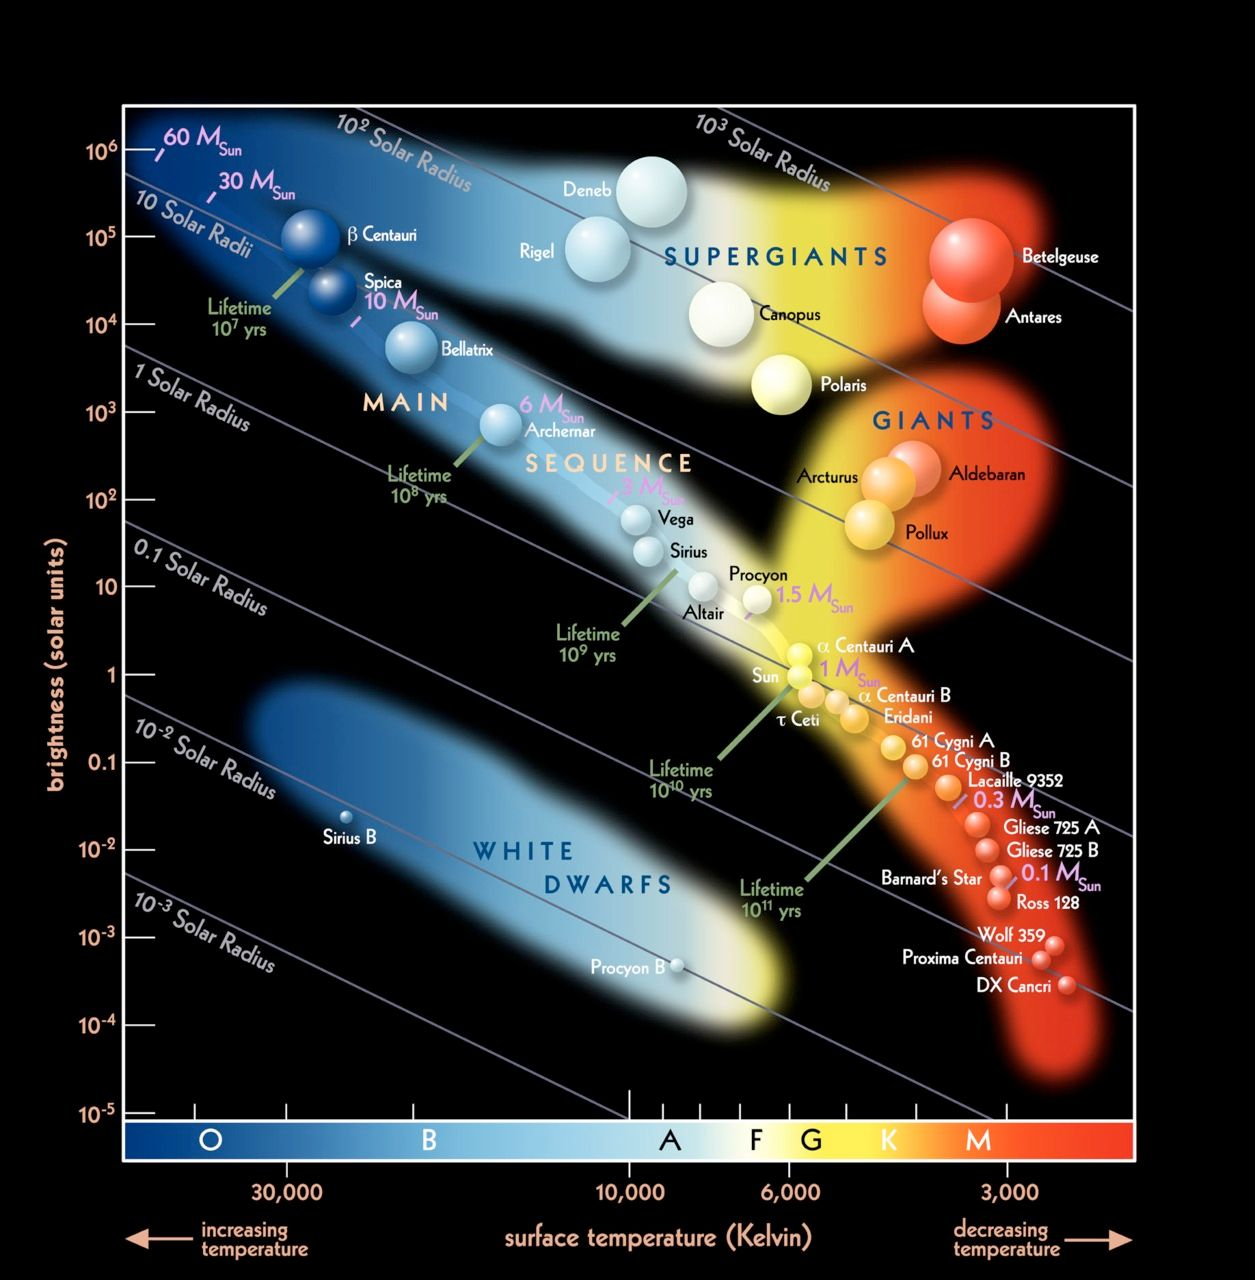
\includegraphics[width=0.65\textwidth]{images/Hertzsprung_Russel_Diagram.jpg}
    \end{center}
    \caption{WRITE CAPTION, INSERT REFERENCE}\label{fig: Hertzsprung_Russel_Diagram}
\end{figure}\\
Since almost all stars go through a phase in the MS, and evolve from there differently, in this work, the chosen starting point for stellar evolution is the Zero Age Main Sequence (ZAMS). 
At this stage, stars have just begun hydrogen burning in their cores, marking the start of their stable main sequence phase.
This allows to bypass the early phases of star formation, which are much less relevant to the gravitational wave sources of interest, while still capturing the essential evolutionary processes that lead to the formation of compact objects.

\subsection{Single star evolution}
Simulating the evolution of a single star is in itself a very complex matter, and the only way to make it computationally feasible in the context of large-scale population synthesis is to approximate the evolution for a wide range of mass $M$ and metallicity $Z$. 
In fact, detailed evolution codes can require substantial computational time even for the evolution of a single star, which is not practical when generating a full-scale astrophysical population containing millions of stars. 
Also, in order to make population synthesis statistically robust a large enough number of stars of a certain type must be evolved in order to overcome stochastic noise (in particular, the Poisson noise for $n$ simulations of a particular type of star, implies an error that grows as $\sqrt{n}$).
A winning strategy, adopted by several population synthesis frameworks, is to pre-generate a large grid of detailed stellar evolution models, and use them to derive a number of interpolation formulae as functions that approximate stellar properties as a function of age, mass and metallicity. 
In \cite{SSE} this method is implemented through the development of a set of \textbf{Single Star Evolution} (\textbf{SSE}) formulae, with the result of a very compact, efficient and adaptable code, which makes it perfect for the integration of binary-star interactions.
The work presented in \cite{SSE} therefore serves as the theoretical and computational foundation for many complex stellar population synthesis codes, including the one used in this thesis. It takes care of the single-star evolution of stars from ZAMS through all the possible evolutionary outcomes, depending on the star's initial conditions.

\subsection{Binary stars evolution}
While the evolution of single stars already represents a challenge, the inclusion of binary interactions introduces a much higher level of complexity.
In such systems, the evolution of each star is strongly influenced by its companion through a variety of processes, such as mass transfer and accretion, common envelope evolution, collisions, supernova kicks, tidal effects, angular momentum loss, and mergers.
These interactions can drastically alter the final outcomes, and are essential for modeling the formation of compact binaries that are potential gravitational wave targets for LISA.
To efficiently model binary evolution within the framework of stellar population synthesis, the work of \cite{BSE} extends the SSE formalism by introducing a set of prescriptions for binary interactions, and updating the treatment of processes such as Roche lobe overflow, common envelope evolution ans coalescence by collision, leading to the development of the \textbf{Binary Star Evolution} (\textbf{BSE}) algorithm.
This code includes the interpolation-based approach used in SSE for single-star evolution, but adds a comprehensive treatment of binary-specific processes, enabling the simulation of a wide range of binary configurations but keeping the affordable computational requirements of SSE.
The BSE algorithm tracks the joint evolution of both stars in a binary system, taking into account their initial parameters, such as masses, orbital period, eccentricity, and metallicity, and updates these properties dynamically as the system evolves.
The flexibility and speed of the BSE code make it a key component in many modern population synthesis tools, including the one used in this thesis, which we will now introduce.

\section{COSMIC}
For the purposes of this work, we employ a community-developed binary population synthesis (BPS) python-based code, called the \textbf{Compact Object Synthesis and Monte Carlo Investigation Code} (\textbf{COSMIC}), whose <<\textit{primary purpose is to generate synthetic populations with an adaptive size based on how the shape of binary parameter distributions change as the number of simulated binaries increases}>>
\footnote{\url{https://cosmic-popsynth.github.io/docs/stable/pages/about.html}}. 
COSMIC's binary evolution is built upon BSE, incorporating extensive modifications in order to include updated physical prescriptions.
It  includes all necessary tools to generate a population, from the generation of initial conditions, to scaling the simulated systems to full-scale astrophysical populations.
The code is presented in \cite{Breivik}, where it is described in full detail and used, as a proof of concept, to simulate the Galactic population of compact binaries and their associated gravitational wave signal.
In the following section we will see the main features of the code, and explain what makes it the right choice for this thesis work.

\subsection{Fixed population}
A fundamental concept in COSMIC, which is the key to the code's efficiency, is the idea of \textit{fixed population}.
This refers to a relatively small sample\footnote{Note that, from now on, every time we talk about sampling, that is where the "M" of COSMIC comes into play: this code uses proficiently the Monte Carlo Markov Chain methods to sample populations and parameter distributions, as will follow in this section.} of just enough binaries to capture, in a statistically meaningful way, the underlying shape of the parameter distribution functions of the target population, as determined by the user specified Star Formation History (SFH) and evolution model.
This is achieved following an iterative process designed to reach a convergence with respect to a defined matching condition, and consists of five key steps:
\begin{enumerate}
    \item The user selects a binary evolution model and SFH;
    \item Based on the SFH and the chosen initial parameter distribution, an initial population is generated;
    \item The population evolves for a user specified number of steps, according to the selected evolution model;
    \item If it is the first iteration, half of the simulated systems is compared with the total population. In the following steps, the population from the previous one gets compared to the population containing both the current and previous iterations.
    In any case, the comparison is done in order to check if the matching condition has been achieved;
    \item Once the parameter distributions of the population have converged, the corresponding population is called \textit{fixed population}, which represents the statistical features of a binary evolution model.
\end{enumerate}
In practice, the fixed population is the converged, computationally efficient representation of the systems that we want to simulate, embedded in a complete small-scale synthetic galaxy that also contains other stellar components.
The output is stored in a data frame, which separates the full galaxy properties from the fixed population ones.
The last step required to construct a full size galaxy is to scale the fixed population (by mass or by number of stars) with a re-sampling approach with replacement, allowing to extrapolate a larger final population that preserves the statistical properties encoded in the fixed population.

\subsubsection{Initialization}
The fixed population is generated from an initial collection of binaries sampled from distribution functions to assign to each binary an initial value of metallicity ($Z$), primary star mass ($m$), mass ratio ($q$), orbital separation ($a$), eccentricity ($e$), and birth time ($T_0$) according to the selected SFH.
In COSMIC the user can choose between different binary parameter distributions, and different parameters can be treated independently.
%In particular:
% \begin{itemize}
%     \item Masses can be sampled from the \cite{Salpeter}, \cite{Kroupa93} or \cite{Kroupa01} Initial Mass Function (IMF);
%     \item Mass ratios are uniformly sampled from \cite{Mazeh92} and \cite{Mazeh94};
%     \item Orbital separations are log-uniformly sampled following \cite{Dominik};
%     \item Eccentricities can be sampled from \cite{Heggie} or from \cite{Geller}; 
%     \item Binarity can follow \cite{Haaften} or follow user specified fractions; 
%     \item COSMIC can also generate initial binary samples following \cite{MoeDiStefano}.
% \end{itemize}
% In this thesis we chose to have independent parameter distributions, and used the default options for all of them, which means \cite{Kroupa01} for the primary model, COMPLETE THIS PART.
Moreover, COSMIC allows a complete personalization of the initial population through a number of other parameters, including different time-steps to control the binary physics, metallicity, stellar winds, common envelope phase, natal kicks, remnant mass, remnant spin, gravitational wave orbital decay, mass transfer, tides, and particular specifications for different kinds of stellar objects, mixing variables, and magnetic braking.
In this work all the parameters were left default, but one: we tweaked the metallicity value, in order to differentiate fixed populations describing the parameter distributions for galaxies of different types.
We will go more into detail on this topic in the next chapters.

\subsubsection{Convergence}
The number of simulated systems in the fixed population ideally describes the final parameter distribution functions while being low enough to keep the code efficient. 
Since every population depends on a different binary evolution model, to quantify this number a \textit{discrete match criteria} is developed, based on the work \cite{Chatziioannou17}.
Independently generated histograms for each parameter are used to track their distribution as successive populations are generated and cumulatively added to the fixed population.
The physical limits of the simulated systems are then enforced by taking the logistic transform, and finally the match is defined as: 
\begin{equation}
    match=\displaystyle\frac{\sum_{k=1}^{N}P_{k,i} P_{k,i+1}}{\sqrt{\sum_{k=1}^{N}(P_{k,i}P_{k,i})\sum_{k=1}^{N}(P_{k,i}P_{k,i+1})}},
    \label{eq: match condition}
    \notag
\end{equation}
where $P_{k,i}$ is the probability for the \textit{k}th bin, for the \textit{i}th iteration.
For how it is defined, the match value shifts between $0$ and $1$, and tends to unity as the parameter distributions converge to a distinct shape.

\subsubsection{The output}
Since COSMIC uses BSE as it’s core binary evolution algorithm, the output of COSMIC follows most of the same conventions as BSE. The \textit{kstar values} (e.g. the number that represent a specific stellar type) and evolution stages are nearly identical to their BSE counterparts, and the exact references can be found in the \textbf{Appendix}.
In order to generate a fixed population, the COSMIC can be ran through a one-line command directly on the terminal, specifying a parameter file, the kstar values for the primary and secondary star, the maximum number of systems to evolve, every how many systems to check in, in order to track the distributions of the parameters, and how many processors to use.
The final output is in an \textit{hdf5} file containing several data frames, that keep track pf various important quantities during the evolution: the total number of stars and total mass of the entire population, the number of binaries, the convergence, and so on. 
The \textit{conv} data frame contains all the information about the final fixed population, and thus is the one that we will use the most: from it we can extract all the parameter distributions of the fixed population, such as the orbital parameters, and the individual star information.
The parameter distributions of a fixed population of binary white dwarfs with a default metallicity value set at $0.020$ is shown in \textbf{Figure~\ref{fig: first fixed pop distributions}}.
\begin{figure}[ht!]
    \begin{center}
        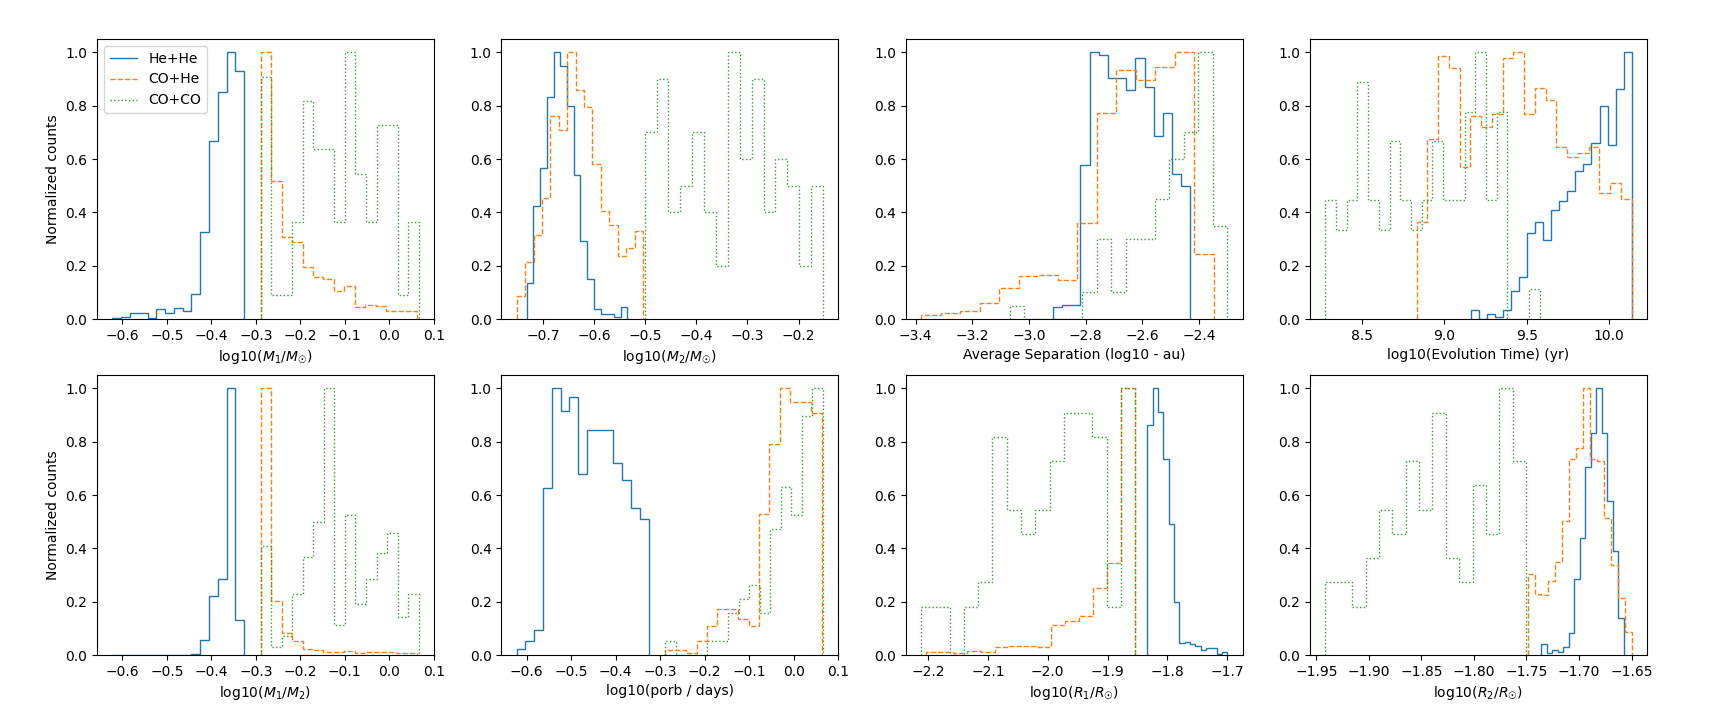
\includegraphics[width=0.85\textwidth]{images/first_fixed_params_distr.jpg}
    \end{center}
    \caption{Distributions of the parameters of a fixed population with metallicity $Z=0.020$ composed of He+He, CO+He and CO+CO binary white dwarfs. This includes the mass, radius of primary and secondary stars, the radius ratios between the two, the orbital period, average separation, and evolution time.}\label{fig: first fixed pop distributions}
\end{figure}



\subsection{Astrophysical population}
Once the convergence criteria is achieved, an astrophysical population can be sampled. 
The number of sources in the astrophysical population $N_{astro, tot}$ can be found by upscaling the size of the fixed population, $N_{fixed}$ ,by the ratio of the mass of the astrophysical population, $M_{astro}$, to the mass of all the stars in the whole small-scale galaxy in which the fixed population is embedded, $M_{fixed,stars}$, as follows:
\begin{equation}
    N_{astro} = N_{fixed}\frac{M_{astro, tot}}{M_{fixed, stars}},
    \label{eq: scale by mass}
\end{equation}
or by the ratio of the number of stars in the astrophysical
population, $N_{astro, tot}$, to the total number of stars formed to produce the fixed population, $N_{fixed,tot}$,
\begin{equation}
    N_{astro} = N_{fixed}\frac{N_{astro, tot}}{N_{fixed, stars}}.
    \label{eq: scale by number}
\end{equation}
Thus, to create a full-scale astrophysical population we need a \textit{reference population} from which we can extract either the total mass or the total number of stars, to then use to scale up our fixed population.
As we will now see, the chosen reference for our purpose is a catalog which reports many key galactic parameters in it, which will allow us to proceed using the method in \eqref{eq: scale by mass}.



\section{GWGC and Galaxy Properties}
As we have seen, the goal of this work is to simulate the gravitational wave background produced by compact binaries in the \textit{local universe}, by generating the sources using COSMIC.
To replicate the existing, observed galaxies in the vicinity of the Milky Way and simulate their stellar content we rely on the dataset provided in \cite{GWGC}, the \textbf{Gravitational Wave Galaxy Catalog} (\textbf{GWGC}).
This catalog includes a list of $53,255$ galaxies within $100Mpc$ from earth, containing information on sky position, distance, blue magnitude, major and minor diameters, position angle, and galaxy type, currently used for follow-up searches of electromagnetic counterparts from gravitational wave searches.

\subsection{What it has vs what we need}
In principle, we could generate a separate fixed population for each galaxy in the GWGC and scale it individually.
However, this is simply not practical because of the computational power and time it would require, and therefore we must find a strategy to group them in a few, representative, categories.
As we will show in this section, many of the information in the GWGC can be used to infer the missing astrophysical quantities we need for population synthesis. 
Ultimately, we will find that metallicity is the most suitable parameter for grouping galaxies.
To get there, we follow a chain of empirical relations, starting from the galaxy morphological type, through  a luminosity to mass, and then a mass to metallicity relation. 
This process will enable us to provide COSMIC with the necessary input, found in a consistent and astrophysically motivated way.



\subsection{Mass-luminosity relation}

As previously discussed, in order to scale a fixed population to the size of a specific galaxy, we need either its total stellar mass or the number of stars.
In particular, \cite{Faber&Gallagher} presents a luminosity-to-mass relation that depends on the morphological type.
This allows to use the blue magnitude and the T-type provided in GWGC to estimate each galaxy's stellar mass.

\subsubsection{Magnitude to luminosity}
To compute the stellar mass, the luminosity-to-mass ratio presented in \cite{Faber&Gallagher} applies to the absolute blue luminosity of each galaxy.
GWGC provides the absolute blue magnitude, thus we have to convert it into blue luminosity using the Sun's blue-band absolute magnitude as a reference (typically $M_{B,\odot} = 5.48$).
Starting from the magnitude definition,
\[
    m_{B,gal} - m_{B,\odot} = -2.5\log_10\left(\frac{L_{B,gal}}{L_{B,\odot}}\right),
\]
which, in stellar units, brings us to the following conversion:
\begin{equation}
    L_{B,gal} = 10^{-0.4(m_{B,gal}-m_{B,\odot})}L_{B,\odot}
    \label{eq: magnitude to luminosity}
\end{equation}
where $m_{B,gal}$ and $m_{B,\odot}\approx 5.48$ are the absolute blue magnitudes of the specific galaxy and the sun.

\subsubsection{Galaxy morphological types}
Although the GWGC denotes galaxy morphology using the de Vaucouleurs T-type scale, the luminosity-to-mass relations used in \cite{Faber&Gallagher} are defined in terms of Hubble morphological classes.
This classification is crucial because different morphological types exhibit significantly different stellar populations and star formation histories, which affect both luminosity and mass content.
For example, elliptical galaxies generally have lower luminosity-to-mass ratios than spirals due to their older stellar populations and lack of ongoing star formation.
Fortunately, a direct correspondence exists between T-type values and Hubble types, and thanks to the results in \cite{Faber&Gallagher} we find the following correspondences:
\begin{table}[h!]
    \centering
    \begin{tabular}{ccc}
        T-Value & Hubble Class & $\frac{M}{L_B}$ \\
        \hline
        $-6.00$ to $-4.01$ & $E$ & 8.5\\
        $-4.00$ to $-2.01$ & $S0^-$ & 9.5\\
        $-2.00$ to $-0.99$ & $S0^+-S_a$ & 6.2\\
        $1.00$ to $3.99$ & $S_{ab}-S_{bc}$ & 6.5\\
        $4.00$ to $4.99$ & $S_{bc}-S_{c}$ & 4.7\\
        $5.00$ to $5.99$ & $S_{cd}-S_{d}$ & 3.9\\
        $6.00$ to $10.00$ & $S_{dm}-Irr$ & 8.5\\
        \hline
    \end{tabular}
    % \caption{Caption}
    \label{tab: mass luminosity conversions tab}
\end{table}\\

\subsubsection{Total mass}
The luminosity resulting from \eqref{eq: magnitude to luminosity}, expressed in units of solar blue luminosity $L_{B,\odot}$, can then be multiplied by the appropriate $M/L_B$ ratio, as in \ref{tab: mass luminosity conversions tab}, to yield the total stellar mass for the galaxy
\begin{equation}
    
    \label{eq: total mass calculation}
\end{equation}


\subsection{Mass-metallicity relation}

    - Finding each galaxy's metallicity from the mass (Tremonti - Allende Prieto)


\section{The final fixed populations}

\subsection{Final catalog editing}

    - Graphs of catalog distributions

\subsection{Metallicity categorization}

    - Metallicity bins for GWGC galaxies, and corresponding fixed populations


\section{Total Gravitational Wave Signal}
- For each galaxy:
    - Compute right $N_astro$
    - compute each binary's GW signal;
    - bin it to LISA's frequency sensibility bins
    - Plot it on LISA's sensibility curve
- Zone of avoidance: how to consider all the sky



\chapter{Results and Discussion}
In the previous chapters, we have laid the theoretical and methodological foundations of our investigation:  
from the gravitational wave theory, to the astrophysical context of white dwarfs and their host galaxies, the principles of gravitational wave detection, and finally the construction of the simulated populations used in this work.  
In this chapter, we turn to the quantitative generation of the corresponding gravitational wave signal.  
We begin by completing the list of galaxies that we use as a reference for the simulations, by taking into account for the incomplete entries of the GWGC and the galaxies obscured by the Zone Of Avoidance.
Afterwards, we generate the fixed populations that are used to simulate all the galaxies, by choosing the corresponding metallicity values based on the range covered by the galaxies in the final catalog.
After discussing LISA's frequency resolution, and understanding how to take it into account, we are able to apply the computational pipeline described in the previous chapter to our final galaxy catalog, extracting the gravitational wave signal from the simulated populations of binary white dwarfs.  
The resulting spectra are then compared to the LISA sensitivity curve to verify the detectability of an extragalactic background.  
Finally, we discuss the frequency distribution and amplitude characteristics of the simulated signals, as well as the physical reasons underlying our results, and their implications for future space-based gravitational wave detectors.


\section{Preparations}
Before computing the total extragalactic DWDs gravitational foreground, we must ensure that our list of galaxies is truly representative of the total population of DWDs in the local universe. 
This means we must consider that the final catalog that we use to compute the signal is incomplete, analysing both the internal and the external causes of lack of galaxies.
Only then, we can group the final galaxies in terms of metallicity, and generate the fixed populations that will be used to reproduce the DWDs hosted in them.
These two steps will lay the ground for the gravitational signal generation and processing.

\subsection{Missing galaxies}
The GWGC is far from being a complete list of the galaxies in the local Universe, and there are two main factors contributing to this: observational limitations due to the Zone of Avoidance (ZOA) and limitations of the information that the catalog presents.

\subsubsection{GWGC incompleteness and non-galactic objects}
The entries of the GWGC represent a source of incompleteness themselves. 
Not all the objects listed in the GWGC are suitable for our purposes:
in addition to galaxies, the catalog also includes globular clusters, which can be identified through their T-type values; 
moreover, not all galaxies in the catalog contain all the information required to perform the procedures described in the previous sections.
To construct a working sample, we applied a series of masks to clean the catalog:
\begin{itemize}
    \item Only keep entries classified as galaxies; 
    \item Require that the distance, T-type, and absolute blue magnitude are provided; 
\end{itemize}
After this selection, the sample we are left with scaled down in size, from the original $53,255$ entries to $20,246$ galaxies suitable for population synthesis.

\subsubsection{Zone of avoidance}
Since the GWGC is an observation-based catalog derived from optical surveys, we must account for the Zone of Avoidance, the region of the sky obscured by the Milky Way’s interstellar dust and stellar crowding, which impedes the detection of background galaxies.
The extent of the ZOA depends on the wavelength of observation: infrared surveys penetrate deeper through the dust, while optical surveys, like those used for GWGC (the reported magnitude for these galaxies is in the B-band), are more strongly affected. 
In the optical band, the ZOA is expected to cover about $\sim25\%$ of the sky, as reported in~\cite{Kraan-Korteweg}.
For this work, we estimated the ZOA directly from the spatial distribution of galaxies in GWGC, by plotting their positions in Galactic coordinates, and highlighting the empty regions of the sky. 
This way, the ZOA appears clearly as a horizontal band centered around the Galactic plane (see \textbf{Figure~\ref{fig: ZOA in galactic coordinates}}).
\begin{figure}
    \begin{center}
        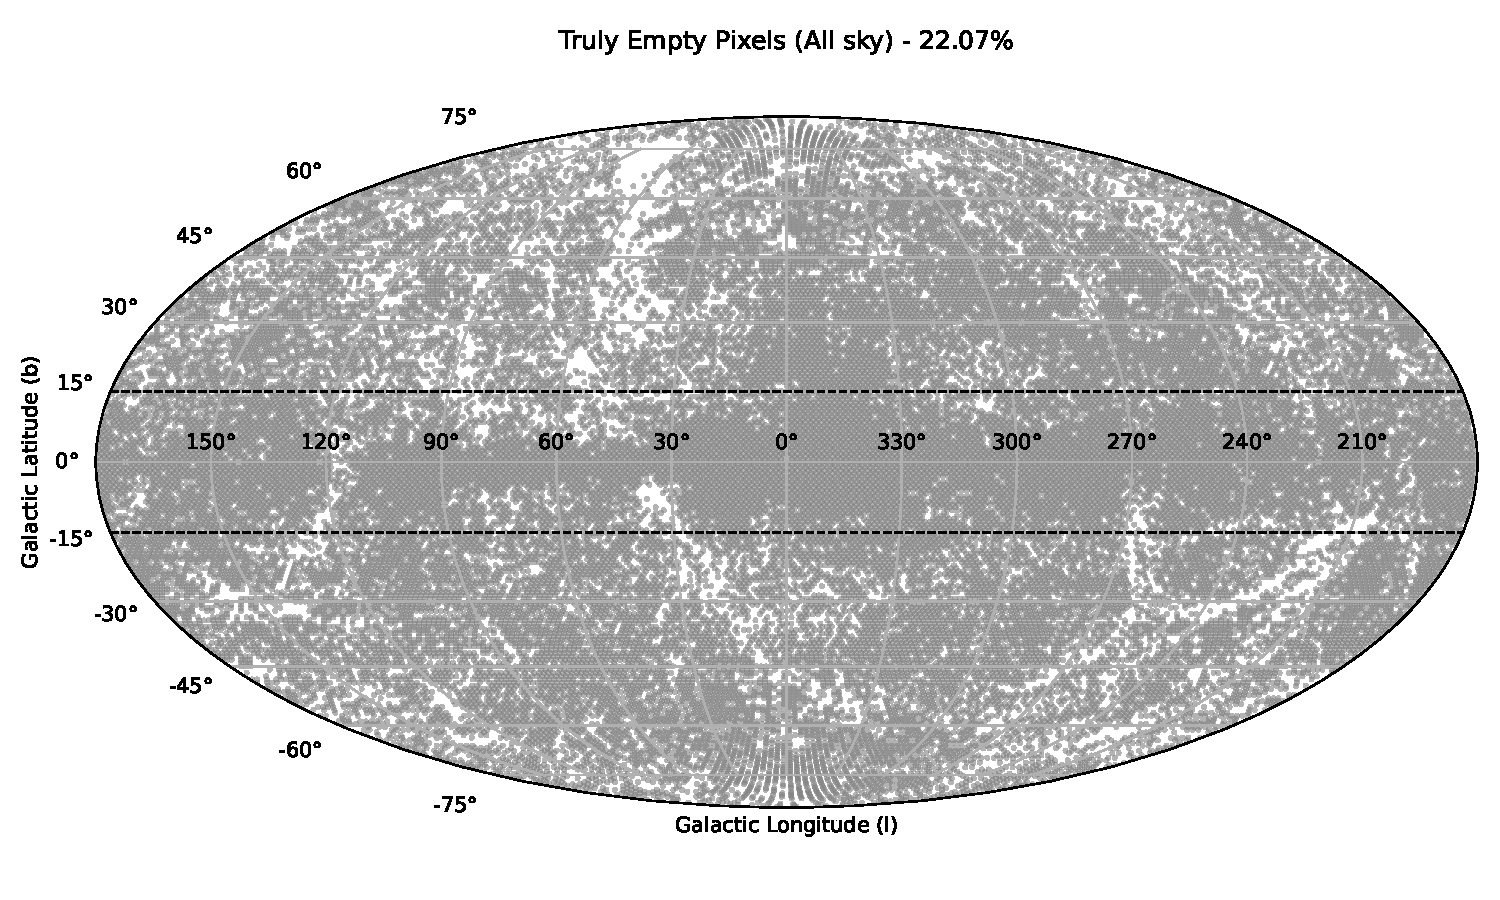
\includegraphics[width=\textwidth]{images/truly_empty_pixels.pdf}
    \end{center}
    \caption{Visual representation of the regions of the sky not covered by any of the 53,255 galaxies in the GWGC, plotted in galactic coordinates using \textbf{healpy}, a Python package that handles pixelated data on the sphere based on the Hierarchical Equal Area isoLatitude Pixelization (\underline{\textbf{\href{https://sourceforge.net/projects/healpix/}{HEALPix}}}). 
    This library allows the user to choose the number of pixels, and thus their size, through a power-of-2 parameter in the \textit{nside2npix} function: the larger the parameter, the smaller the pixel and the bigger their number. 
    The gray dots in the figure represent the empty sky pixels, while the white areas correspond to pixels containing at least one galaxy.
    The central band, where the Milky Way lies, appears significantly emptier than the rest of the sky; this is the so called Zone Of Avoidance (ZOA).
    To estimate the ZOA, we calculated the percentage of empty pixels in the band $|b| \leq 15^\circ$ in Galactic latitude.
    Choosing the parameter to be too small, the produced pixels would be too large, and the empty area would be underestimated.
    Larger values would make the estimation only more precise, and by selecting parameters starting from $2^6=64$, it's possible to estimate roughly $\sim20\%$–$25\%$ of empty sky, fully consistent with the value reported in~\cite{Kraan-Korteweg}.
    The $22.07\%$ estimation in the title is found using $64$ as parameter value.
    }\label{fig: ZOA in galactic coordinates}
\end{figure}
To quantify its extent, we used a Python package that handles pixelated data on the sphere based on the Hierarchical Equal Area isoLatitude Pixelization, \underline{\textbf{\href{https://sourceforge.net/projects/healpix/}{HEALPix}}}, called healpy, to divide the sky map into $n_{\rm pix}$ equal-area pixels, and focused on the band $|b| \leq 15^\circ$ in Galactic latitude.
Counting the empty pixels in this band and dividing by $n_{\rm pix}$ gives an estimated ZOA coverage of $\sim20\%$–$25\%$ of the sky, depending on the chosen pixel resolution.
This estimate is fully consistent with the literature~\cite{Kraan-Korteweg}, so in our analysis we will assume that GWGC effectively covers $\sim80\%$ of the sky.

\subsubsection{Filling the gap}
In order to compensate the missing galaxies, we have made two physically motivated assumptions.
\begin{enumerate}
    \item \textbf{Cosmological Principle}:\\
    The GWGC lists all the observed galaxies within $100Mpc$.
    On such scales, the Universe can be assumed to be statistically \textit{homogeneous} and \textit{isotropic}. 
    This assumption is supported from observations of the \textit{Cosmic Microwave Background} (CMB), where we know that the correlation function of the temperature fluctuations across the sky peaks at scales of $\sim100Mpc$. 
    Under this assumption, the selected galaxies of the GWGC should be statistically representative of the overall population in the same volume, and therefore of the missing galaxies too.
    \item \textbf{Distance}:\\ 
    The angular position is irrelevant in the computation of the gravitational wave signal: only the distance of the source matters.
    Therefore, missing galaxies from the unexplored volume covered by the Milky Way can be statistically represented by the galaxies from our retained sample.
\end{enumerate}
Following these assumptions, we “fill in” the missing fraction of the sky and the dropped entries of the catalog by sampling with replacement from the cleaned GWGC, just like we did to extract an astrophysical population from the fixed one, preserving its parameter distributions.
This ensures that the statistical properties of the synthetic galaxy distribution match those of the observed portion while restoring the full-sky coverage. 
This is shown in a graphical representation of the distributions of distances, blue band magnitudes and T-types, in \textbf{Figure~\ref{fig: distro comparison}}: the distributions have been scaled up without visible changes.
\begin{figure}[h!]
    \begin{center}
        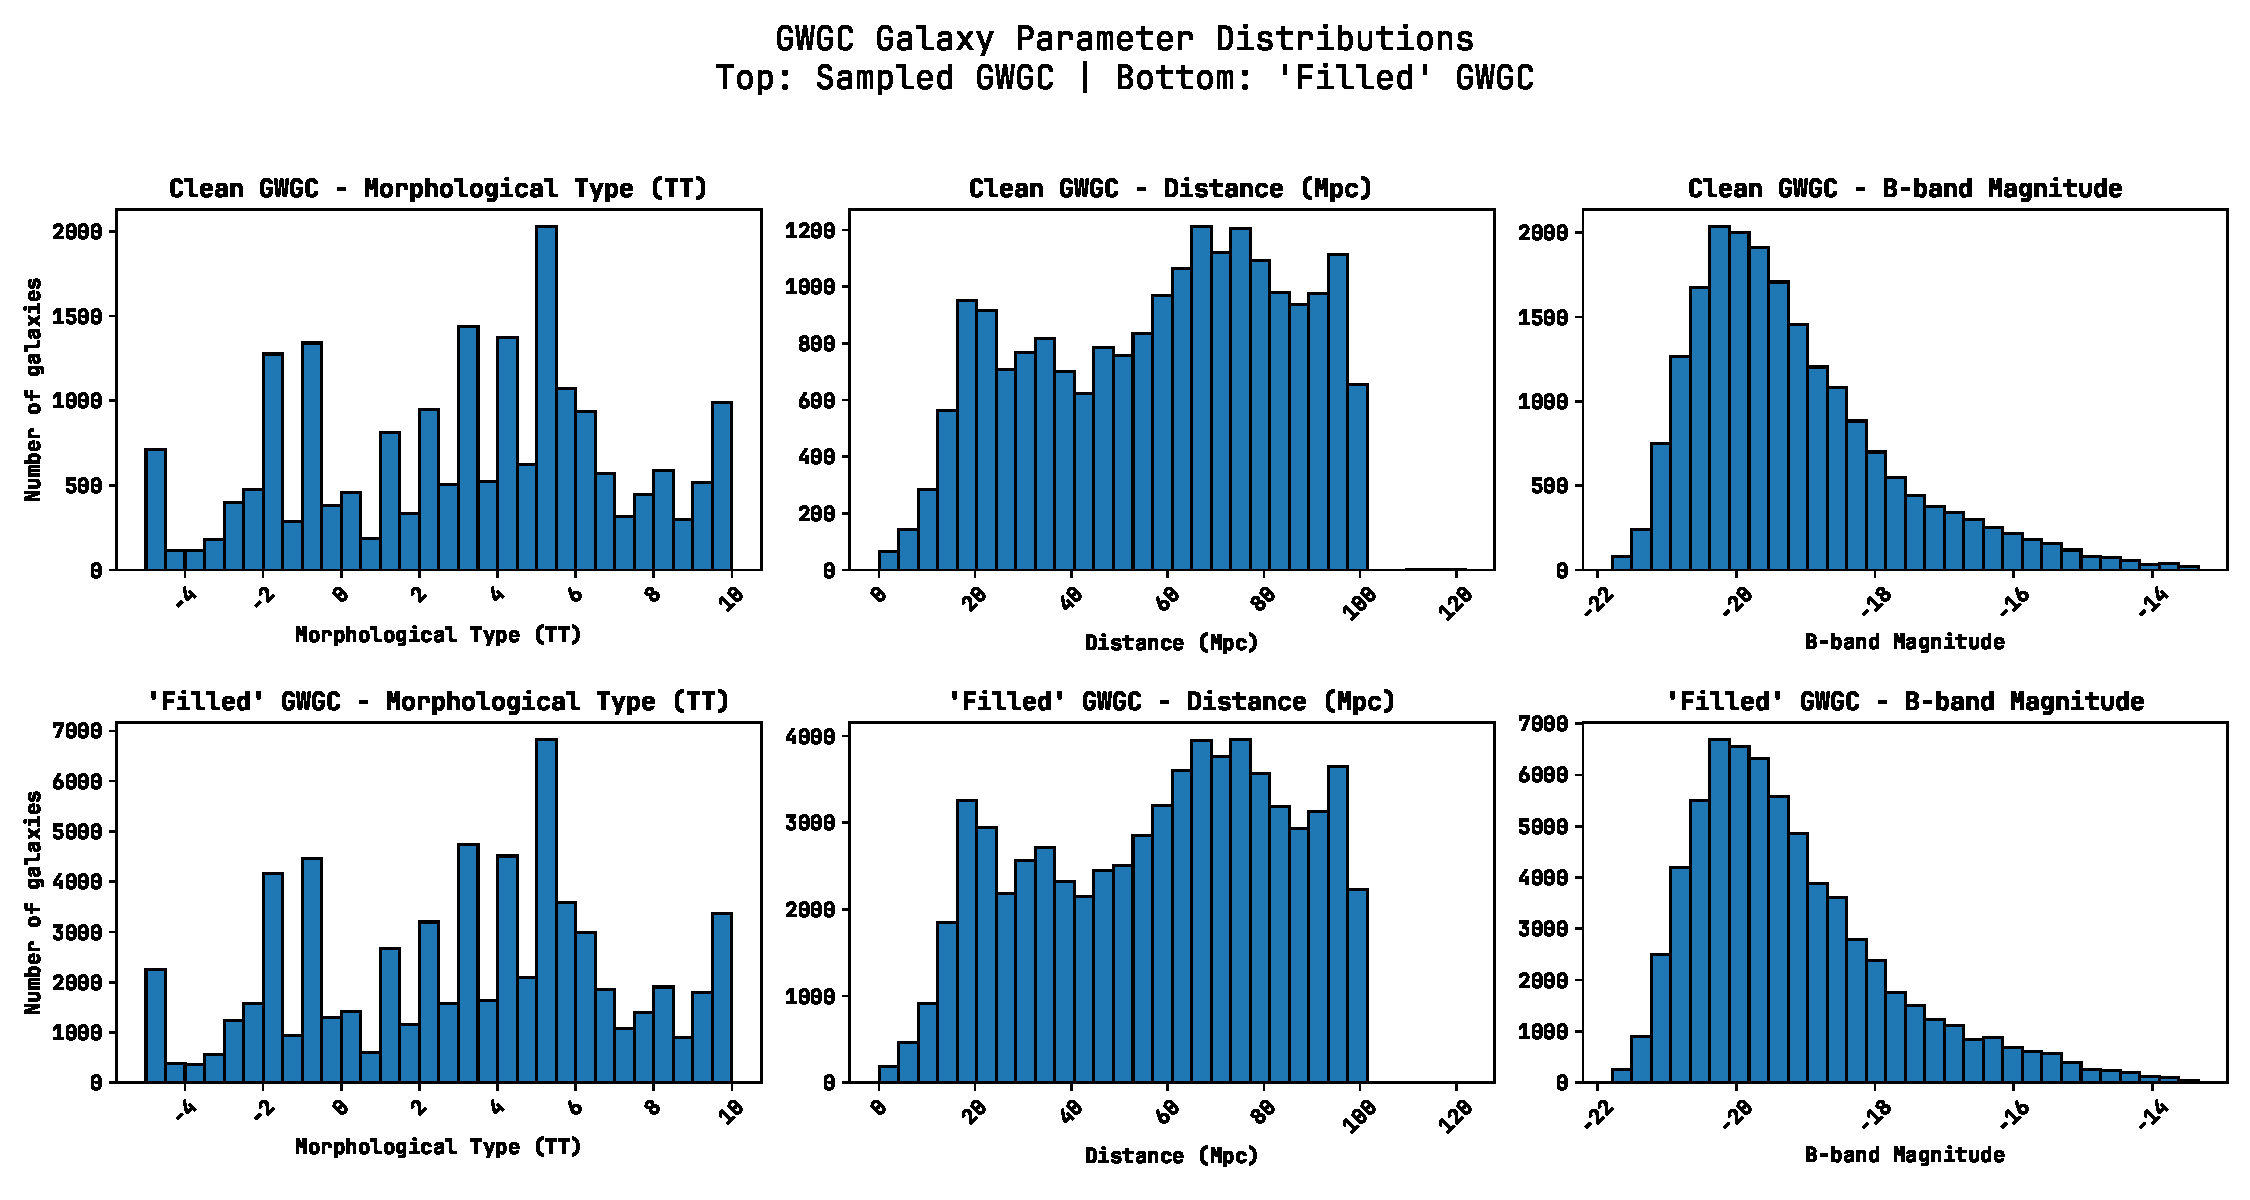
\includegraphics[width=\textwidth]{images/distro_comparison.pdf}
    \end{center}
    \caption{Distributions of T-type, distance and B-band magnitude of the galaxies in the \textbf{Gravitational Wave Galaxy Catalog} (\textbf{GWGC}) before and after compensating for the lack of galaxies due to the catalog's incompleteness and the \textbf{Zone Of Avoidance} (\textbf{ZOA}). 
    The three graphs \textit{above} show the mentioned distributions for the $20,246$ galaxies of the original GWGC after we dropped those missing the key parameters we needed; the three graphs \textit{below} show the same distributions for the $66,568$ galaxies we are left with after taking into account both the catalog's incompleteness and the ZOA using a sampling with replacement method.
    The parameters distributions appear to be indistinguishable in shape: the scaling up in size left the properties of the catalog unchanged.
    }\label{fig: distro comparison}
\end{figure}
\\
The total number of galaxies that we have after taking into consideration both the dropped incomplete entries of the original GWGC and the galaxies covered by the ZOA, has grown to $66,568$.


\subsection{The final fixed populations}
As we already discussed, the metallicity of a galaxy has a great impact on the stellar evolution and, thus, on the gravitational wave signal.
This, plus the fact that metallicity is also closely linked to the galaxy types, led us to choose it as characterizing parameter for the fixed populations that we will generate to represent the galaxy in the catalog.
In particular, we the final catalog covers a range from a minimum of $ Z_{min}= 0.00748$ to a maximum of $Z_{max}= 0.03948$.
We decided to group all the values in between in ten equally wide bins, represented in \textbf{Figure~\ref{fig: Z distribution of final catalog}}.
\begin{figure}[h!]
    \begin{center}
        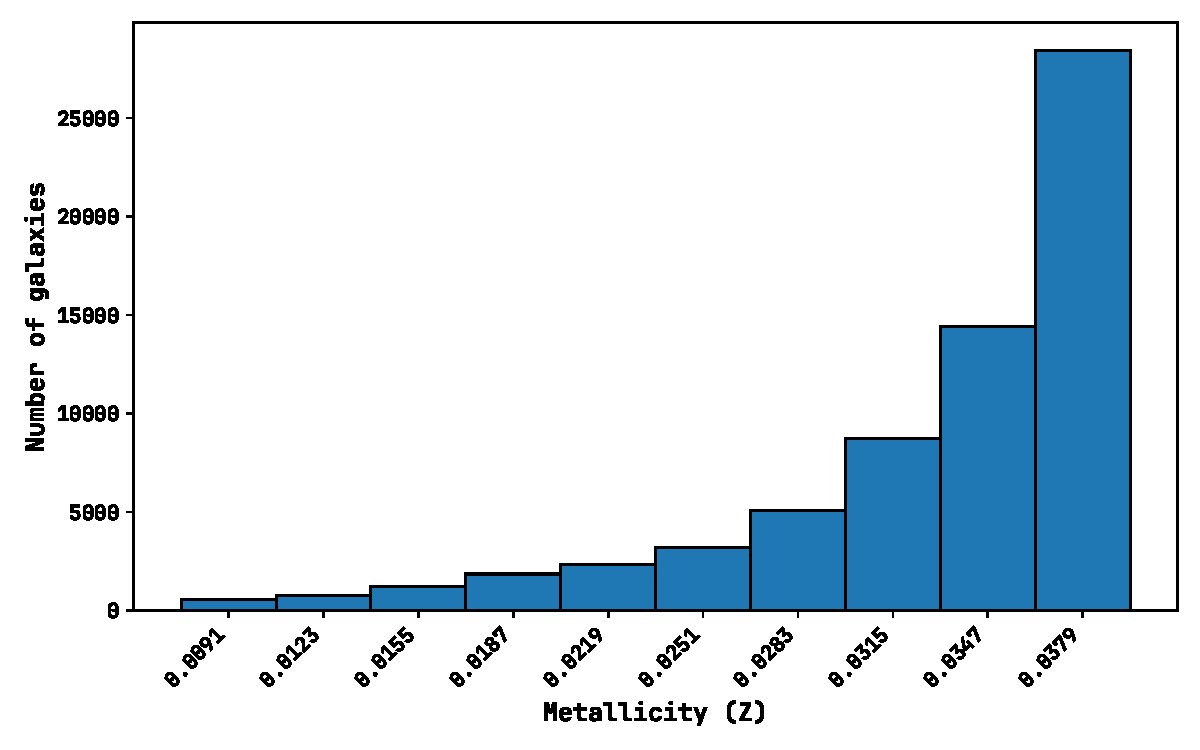
\includegraphics[width=\textwidth]{images/z_distro_gwgc_completed_ZOA.pdf}
    \end{center}
    \caption{Metallicity distribution of the final galaxy catalog. 
    The metallicity of the galaxies has been shown to correlate with their morphological type in~\cite{Faber&Gallagher}.
    Therefore, the entries of our final catalog can be grouped into 10 bins, each associated to a metallicity value (the middle value of the corresponding bin, shown in the $x$-axis label of the graph), and a corresponding fixed population.
    }\label{fig: Z distribution of final catalog}
\end{figure}\\
Each one of the bins center values, shown in the $x$ label, is linked to a different synthetic fixed population generated with COSMIC.
The simulations were done generating the fixed populations "\textit{\href{https://cosmic-popsynth.github.io/docs/stable/pages/fixedpop.html}{the cosmic way}}", via terminal, specifying $Nstep = 5000$ and $Niter=1000000000$ and kstar values $10$, $11$ and $12$, corresponding to He, CO, and Ne white dwarfs\footnote{All the kstar values and the corresponding astrophysical objects are shown in \textbf{Table~\ref{tab: kstar values}}, in the \textbf{Appendix}.}, assuming the sun's metallicity to be $Z_\odot = 0.0134$ and leaving all the remaining COSMIC's specifiable parameters unchanged from the default values.


\section{The Signal Computation}
Generating the DWDs using COSMIC gives us the possibility to calculate the gravitational wave contribution of each one of them, assuming their distance to be the same as the hosting galaxy's one, provided from the galaxy catalog, and with an extreme precision in frequency.
Before scaling up the fixed population, and calculating each binary's gravitational wave signal, and confronting it with LISA's sensitivity curve, we must then consider LISA's limited \textit{frequency resolution}, and understand how to process the signals of indistinguishable sources.

\subsection{LISA's frequency resolution}
The duration of LISA’s mission directly impacts its frequency resolution: the longer the observation time, the finer the frequency bins it can resolve.
In this work, we assume an observation time of: 
\[
    T_{obs}=4yr=126,144,000s
\]
which corresponds to a minimum frequency resolution of
\begin{equation}
    \delta\nu_{LISA,\min}\approx \frac{1}{T_{obs}}\sim 8\times 10^{-9}Hz.
    \label{eq: LISA frequency resolution}
\end{equation}
This fundamental limit comes from the Fourier transform properties, and determines the smallest frequency interval over which the signals can be resolved.
Although this is a very fine resolution, the precision of the orbital period in the simulated binary systems, and thus the frequency resolution on their gravitational signal, is actually much bigger, since these values come from a simulation rather than from real observations.
For this reason, when computing the gravitational wave signals of our simulated binaries, we must take into account the fact that LISA will not be able to distinguish sources within the same frequency bin.
To model this, we group the resulting gravitational wave signals in bins of size $\delta\nu_{LISA,\min}$, and sum all the signals that fall within each bin.

\subsubsection{Signals summation}
In principle, over the observation time $T_{obs}$, the orbital parameters of the sources may slowly evolve, causing a drift in the gravitational wave frequency. 
Integrating the resulting signal during this period is no easy task.
However, for the slowly evolving white dwarf binaries we are considering, the change in such short time-frames is negligible, so we can treat their signals as effectively monochromatic within the observation window. 
Thus, we can define a commonly used variable to simplify our job, which is called  \textbf{Amplitude Spectral Density} (\textbf{ASD}):
\begin{equation}
    ASD = h\sqrt{T_{obs}},
    \label{eq: ASD definition}
\end{equation}
where $h$ is the gravitational wave strain of the binary, computed in~\eqref{eq: the strain we use}, and $T_{obs}$ is the mission duration for LISA.
This quantity represents the characteristic strain amplitude of the gravitational wave signal per square root of frequency, scaled by the observation time, and its very convenient for comparing the signals in frequency space.
Correspondingly, we can define the \textbf{Power Spectral Density} (\textbf{PSD}) as the square of the ASD
\begin{equation}
    PSD = ASD^2,
    \label{eq: PSD definition}
\end{equation}
which properly represents the signal power per frequency unit.
Since power contributions from independent sources add linearly, the total PSD in a given frequency bin is simply found by summing the power of all the sources within it:
\begin{equation}
    PSD_{tot,bin_1} = PSD_{*_1,bin_1} + PSD_{*_2,bin_1} + \dots
    \label{eq: total PSD}
\end{equation}
This way, we effectively accounted for LISA's frequency resolution limit.
The reason for introducing this quantities is that gravitational waves from different binaries are uncorrelated, so their strains add incoherently. 
This means that we cannot simply sum the strain amplitudes directly.
Instead, the PSD provides a way to combine signals that ensures a correct representation of the combined gravitational wave background.

\subsection{The pipeline}
In order to compute the total extragalactic DWDs gravitational background, we must apply an iterative process to each galaxy in the final catalog, which consists of the following steps:
\begin{itemize}
    \item Compute the right $N_{astro}$ using the~\eqref{eq: scale by mass}
    \item Scale the fixed population accordingly with a sampling with replacement method, creating the full-size galaxy simulation.
    \vspace{1.5mm}\\
    At this point for each binary system in this astrophysical population we:
    \begin{itemize}
        \item Compute the gravitational wave signal using~\eqref{eq: the strain we use}\footnote{Note here that all the binaries within the same galaxy are given the same distance from us. This approximation is considered to be valid since the distance of the galaxy is much much bigger then its size, and thus then the maximum possible distance between two binaries within the same galaxy.} and the corresponding $PSD$ using~\eqref{eq: ASD definition} and~\eqref{eq: PSD definition};
        \item Sum the total PSD of the binaries whose frequencies fall within the same LISA's frequency bin, using~\eqref{eq: total PSD};
        \item Plot the total binned signals on LISA's curve.
    \end{itemize}
\end{itemize}
\subsubsection{LISA's sensitivity curve}
The LISA curve is constantly updated when new gravitational wave components that can affect it are found, meaning that there are many different versions around.
The one we chose to adopt is the widely used version presented in~\cite{Robson_2019}, which is written as:
\begin{equation}
    S_n = \frac{10}{3L^2} \left( P_{OMS}(f) + \frac{4P_{acc}(f)}{(2\pi f)^4} \right)\left( 1 + \frac{6}{10}\left(\frac{f}{f_*}\right)^2 \right) + S_c(f),
    \notag
    %\label{eq: LISA sensitivity curve by Robson}
\end{equation}
where $L=2.5 Gm$ is the LISA arm length, $f_*=19.09mHz$ and $P_{OMS}(f)$, $P_{acc}(f)$ and $S_c(f)$ are the expressions for the single-link optical metrology noise, the single test mass acceleration noise and the total Michaelson-style LISA data channel. 
The equations for these factors, as well as more detail on the curve, can be found in the article.


\section{Discussion}

Doing this, the spectral distribution of the final resulting signal is plotted over the LISA's sensitivity curve\footnote{This particular curve is presented in~\cite{Robson_2019}.} in \textbf{Figure~\ref{fig: Final results plot}}.
\begin{figure}[ht!]
    \begin{center}
        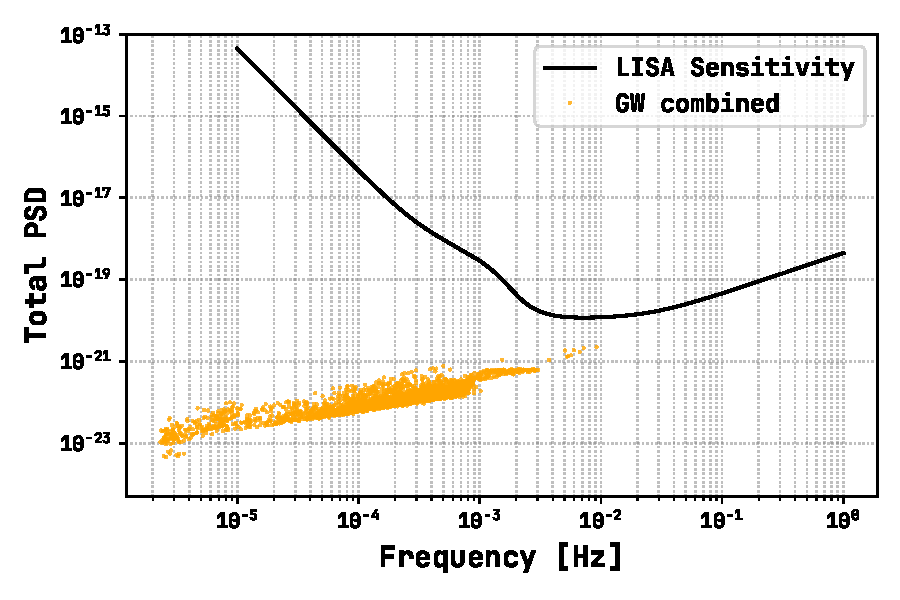
\includegraphics[width=\textwidth]{images/Final_results_plot.pdf}
    \end{center}
    \caption{Total gravitational wave signal of the simulated Double White Dwarfs (DWDs) hosted by the $66,568$ galaxies of the final catalog, binned in $\sim 8\times10^{-9}Hz$ large frequency bins, representing LISA's spectral resolution for an observational time $T_{obs}\sim4yr$. 
    Every orange dot represents the signal of a frequency bin, calculated by summing the Power Spectral Density (PSD) of every galaxy that it contained, using~\eqref{eq: total PSD}. 
    The dots are plotted on LISA's sensitivity curve, as found in~\cite{Robson_2019}, and appear to be about one order of magnitude below the minimum threshold of this curve.
    This results suggest that we should not expect LISA to be able to detect the unresolved extragalactic DWDs confusion foreground, at least under the assumptions and approximations adopted in this work.}\label{fig: Final results plot}
\end{figure}
Every orange dot in this graph represents a frequency bin, whose width is given by~\eqref{eq: LISA frequency resolution}, where the gravitational wave signal of all the binaries within it has been summed using~\eqref{eq: total PSD}.
The resulting calculated signal appears to be about one order of magnitude smaller than the minimum detectable strain for LISA across the whole band.  
This indicates that, luckily, the stochastic contribution from unresolved extragalactic DWDs will not have a measurable impact on LISA’s sensitivity curve, at least under the assumptions of our population model and scaling relations. 

\paragraph{Distribution of the sources}
The simulated extragalactic binaries foreground populates primarily the low-frequency range ($f \lesssim 2\,\mathrm{mHz}$), with the number of systems per frequency bin increasing steeply at higher frequencies. 
This is evident for at least two reasons:
\begin{enumerate}
    \item The orange dots seem to be more sparse at lower frequencies, and increasingly densely packed towards higher frequencies, showing that more empty bins appear to be at the lower end of the spectrum, and the more populated ones at the higher end;
    \item The sources appear to lay on a slope, with the PSD values steadily increasing with the frequency, showing that at higher frequencies, the occupied frequency bins tend to be more and more populated, and therefore the total PSD they contain higher and higher in magnitude.
\end{enumerate}
A possible physical explanation for this phenomenon is that the time evolution of the orbital parameters is initially very slow, allowing the orbital frequencies to distribute over a wider range of bins.
As the binary systems evolve they get more compact, and the parameters change more rapidly, increasing the likelihood that the systems occupy very close frequency bins.
Moreover, the spectral shape of the resulting background is positioned at frequencies that are similar to the expected Galactic foreground ones (corresponding to the slight bump at the left of the lowest point in the graph. 
This is better shown in \textbf{Figure~\ref{fig: LISA sens curve with noises}}), but with a significantly lower amplitude due to the much larger average distances.
Indeed, as shown in~\eqref{eq: the strain we use}, the gravitational wave amplitude scales inversely with the distance from the source, so even relatively nearby galaxies contribute far less per binary than the Milky Way population. 
The total number of galaxies in the local Universe, even if large, is not sufficient to compensate for this distance-induced amplitude suppression.


\subsection{Stability of the results}
The simulated gravitational wave signal, represented by the orange dots, would be detectable by LISA if it fell above the LISA curve, meaning that the total PSD in a certain frequency bin is higher than the minimum threshold of LISA's sensitivity.
Therefore, the dots can get close to, or above the sensitivity curve either by containing extremely close and strong sources, by containing the contribution of many farther, and fainter sources, or a combination of both.
In principle, the results we presented could depend on the assumptions we made, and the methods we used.
In particular, for what we have just said, the most important steps we took in this regard are and the calculation of the signal, and the representation the sources.

\subsubsection{The sources}
The results could be affected by the way we represented the sources, via GWGC.
Indeed, this is the input we give our pipeline to produce, as an output, what should be the total gravitational wave confusion foreground from all the unresolved DWDs in the local universe.
For example, if we only used the GWGC catalog after dropping the incomplete voices, and without considering the zone of avoidance, the total gravitational wave signal produced by the remaining $20,246$ galaxies would be as represented in \textbf{Figure~\ref{fig: total signal plot with incomplete catalog}}.
\begin{figure}
    \begin{center}
        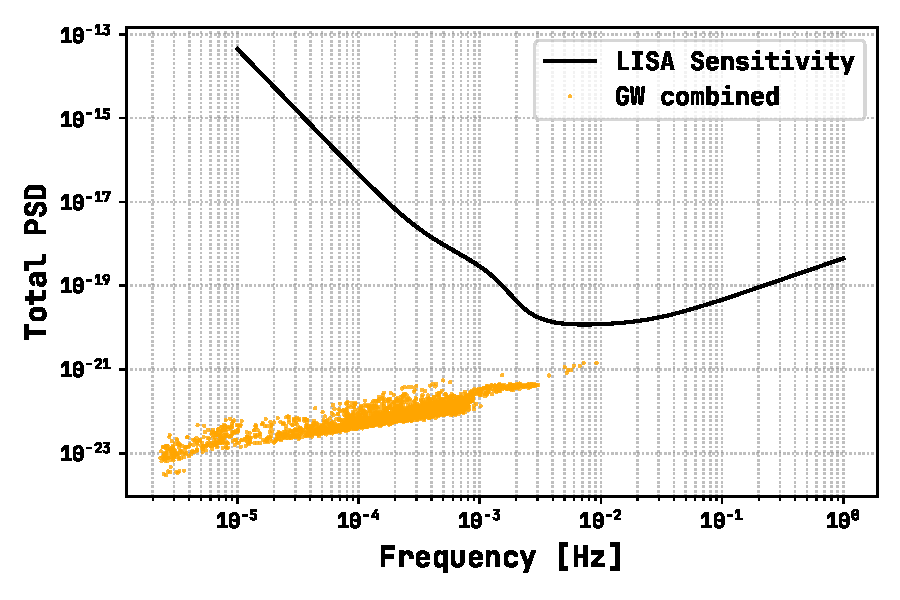
\includegraphics[width=\textwidth]{images/Final_results__incomplete_GWGC_plot.pdf}
    \end{center}
    \caption{Total gravitational wave signal of the simulated Double White Dwarfs (DWDs) hosted by the $20,246$ galaxies of the GWGC after dropping the galaxies with incomplete information, and without considering the zone of avoidance. 
    The signal is binned in $\sim 8\times10^{-9}Hz$ large frequency bins, representing LISA's spectral resolution, assuming an observational time $T_{obs}\sim4yr$. 
    Every orange dot represents the signal of a frequency bin, calculated by summing the Power Spectral Density (PSD) of every galaxy that it contained, using~\eqref{eq: total PSD}. 
    The dots are plotted on LISA's sensitivity curve, as found in~\cite{Robson_2019}, and appear to be about one order of magnitude below the minimum threshold of this curve.
    This results, if compared with the ones showed in \textbf{Figure~\ref{fig: Final results plot}}, show that the effect of not taking into account the missing galaxies is very small, barely noticeable. 
    }\label{fig: total signal plot with incomplete catalog}
\end{figure}
Although a slight difference in height with the results obtained for all the $66,568$ galaxies presented in \textbf{Figure~\ref{fig: Final results plot}} is noticeable, it is important to note that it is caused by considering less then a third of the sources.
Therefore, even if it is possible to consider different and more complete catalogs, and the zone of avoidance could be estimated with better precision, the results we found do not depend significantly on this.
In addition to this, the single DWDs were simulated using COSMIC, which represent and arbitrary choice between a number of different population synthesis codes: a different code might produce different sources parameter distributions, and could be an interesting extension of the present work.

\subsubsection{The signal}
The main assumptions we made to obtain the results are surely how we calculated the gravitational wave characteristic strain, and the way we integrate the signal coming from unresolved sources within the same frequency bin.
The gravitational wave signal calculated in~\eqref{eq: the strain we use} is the standard characteristic strain predicted from the General Relativity for an inspiraling binary system, and is therefore the most precise way to represent the DWDs signal.
Furthermore, the use of Amplitude Spectral Density (ASD) and Power Spectral Density (PSD) is unavoidable, since it is the only way to confront signals that LISA could not resolve in frequency with its sensitivity curve.
Interestingly, assuming a longer observational time would guarantee LISA a better frequency resolution, and each frequency bin would appear to be less populated.
Since, as we said, less populated bins generally contain lower total PSD, the better the LISA's frequency resolution, the lower the sensitivity to the noise that the unresolved sources produce, and therefore the lower LISA's sensitivity curve needs to be to detect it.
Overall, the methods we used guarantee a pretty stable and reproducible output, given the same input.



\chapter*{Conclusions and Future Perspectives}
\addcontentsline{toc}{chapter}{Conclusions and Future Perspectives}
In this thesis we investigated the contribution of extragalactic double white dwarf (DWD) binaries to the low-frequency gravitational wave (GW) background, with a focus on their potential detectability by the space-based interferometer LISA.  
We began by discussing the theoretical gravitational wave framework, and the astrophysical elements that are relevant to this problem, including a brief description of the formation and evolution of white dwarfs, both as isolated stars and in binary systems, and the galactic environments in which they reside and evolve. 
We then discussed the fundamentals of interferometric detection, and the specific capabilities of LISA as a space-based detector.  
On this theoretical basis, we developed a computational pipeline to simulate synthetic populations of extragalactic DWD binaries using the population synthesis code COSMIC. 
We then scaled them according to the stellar masses of host galaxies, using the astrophysical observations galaxy survey "\textit{Gravitational Wave Galaxy Catalog}" as reference, and computed their GW strain and power spectral density. 
The simulated signals were finally binned according to LISA’s frequency resolution and compared with its sensitivity curve.
The main result of this study is that the predicted gravitational wave signal from the extragalactic DWD population lies approximately one order of magnitude below LISA’s detection threshold, as found in \cite{Robson_2019}, across the considered frequency band.  
Therefore, although, as we know, DWD binaries are expected to constitute a dominant foreground from Galactic sources, able to shape LISA's curve substantially, the extragalactic component is not expected to measurably affect it at all.
While the present analysis points towards a negligible extragalactic contribution for LISA, it provides a quantitative baseline that can be refined in several directions.  
For example, future work could incorporate more detailed galaxy catalogs with redshift-dependent star formation histories and metallicity evolution, and that take in account more precisely the missing sources blocked from our Galaxy in the \textit{Zone Of Avoidance}.
Similarly, improving the binary population synthesis models, for example by including different prescriptions also on other parameters, and not only focusing on the metallicity, like mass transfer prescriptions or alternative common-envelope outcomes.
Moreover, since population synthesis is a very active and rapidly evolving research field, testing alternative codes, possibly based on different Single Star and Binary Stars evolution models, could help quantify the model dependence of our predictions and reveal systematic uncertainties.
Finally, although the extragalactic DWD background may be undetectable for LISA, this work shows how future space-based detectors with longer baselines or improved sensitivity in the sub-millihertz regime could, in principle, probe this population, offering a complementary view to Galactic studies and providing constraints on the binary evolution across cosmic time.
In summary, this work has explored a previously the extragalactic DWDs component of the GW landscape, reinforcing the understanding that the gravitational wave sky at low frequencies will be dominated by Galactic sources, but also highlighting that the extragalactic background, though faint, remains a scientifically interesting target for the next generation of detectors.


\appendix

\chapter{}
\begin{table}
    \caption{In this table are presented all the possible kstar values that the user can choose in COSMIC, and the corresponding astrophysical object and evolutionary state.}\label{tab: kstar values}
    \begin{center}
        \begin{tabular}[]{l|l}
            \toprule
            \multicolumn{1}{c|}{\textbf{kstar value}} & 
            \multicolumn{1}{c}{\textbf{evolutionary state}} \\
            \midrule
            0 & Main Sequence (MS), $< 0.7 M_\odot$ \\
            1 & MS, $>0.7 M_\odot$ \\
            2 & Hertzsprung Gap \\
            3 & First Giant Branch \\
            4 & Core Helium Burning \\
            5 & Early Asymptotic Giant Branch (AGB) \\
            6 & Thermally Pulsing AGB \\
            7 & Naked Helium Star MS \\
            8 & Naked Helium Star Hertzsprung Gap \\
            9 & Naked Helium Star Giant Branch \\
            10 & Helium White Dwarf \\
            11 & Carbon/Oxygen White Dwarf \\
            12 & Oxygen/Neon White Dwarf \\
            13 & Neutron Star \\
            14 & Black Hole \\
            15 & Massless Remnant \\          
            \bottomrule
        \end{tabular}
    \end{center}
\end{table}


% \chapter{}
% Dettagli tecnici sul codice.
% 
% Tabelle di parametri.
% 
% Ulteriori grafici.
% 
% Script di calcolo, se rilevante.


%\chapter{Questa è un'appendice}

%\lipsum[5]

%\section*{Questa è un'altra sezione, ma non viene inserita nell'indice}

%\lipsum[6]

%\bibliography{chapters/Bibliografia}
\nocite{*}
\bibliographystyle{plainnat}
\bibliography{chapters/Bibliografia.bib}

\end{document}
% -----------------------------------------------------------------

